\documentclass{beamer}
\usepackage{beamerthemesplit} % new

\usepackage[utf8]{inputenc}
\usepackage{tikz}

\newcommand{\roundpic}[4][]{
  \tikz\node [circle, minimum width = #2,
    path picture = {
      \node [#1] at (path picture bounding box.center) {
        \includegraphics[width=#3]{#4}};
    }] {};}

\usepackage{graphicx,wrapfig,lipsum}
\usepackage{multicol}

\usepackage{tcolorbox}






\begin{document}
\title{MY-NEIGH}
\author{BDBI\_2019\_GR\_04}
\date{\today}

\frame{\titlepage}

\frame{\frametitle{Table of contents}\tableofcontents}


\section{Team Members}


    
\frame{\frametitle{Team}
  \begin{itemize}
    \item MARTA IBÁÑEZ 
    \item JUDIT CAMPS   
    \item AINA MONTALBAN 
  \end{itemize}
  \vspace{1cm}
  \hspace{2cm}
 \roundpic[xshift=-0.03cm,yshift=-0.03cm]{2cm}{2cm}{images/marta.png}
   \hspace{0.5cm}
 \roundpic[xshift=-0.03cm,yshift=-0.03cm]{2cm}{2cm}{images/judit.JPG}
    \hspace{0.5cm}
  \roundpic[xshift=-0.03cm,yshift=-0.03cm]{2cm}{2cm}{images/aina.JPG}


}

\section{Project}
\frame{\frametitle{Project Description}
\begin{tcolorbox}[colback=blue!5,colframe=blue!40!black,title=Purpose]
Management of neighbourhood associations (NA).
\begin{itemize}
\item Property administrator (PA)
\item Neighbours
\end{itemize}
\end{tcolorbox}
\hspace{4.4cm}

\includegraphics[scale=0.3]{images/PA-2.png}

\includegraphics[scale=0.3]{images/PA-3.png}

\includegraphics[scale=0.3]{images/PA-4.png}

\includegraphics[scale=0.3]{images/PA-5.png}

}

\section{Trello}
\subsection{Trello Tasks}
\frame{\frametitle{Plan}
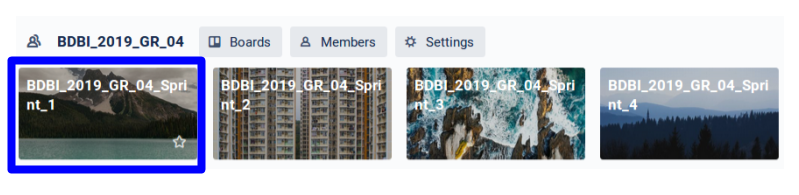
\includegraphics[scale=0.37]{images/trello-02.png}\\
\hspace{0.2cm}
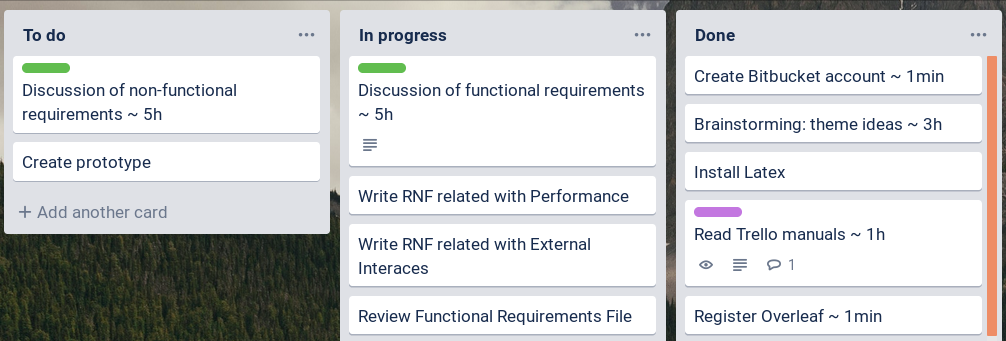
\includegraphics[scale=0.27]{images/trello-04.png}
}

\frame{\frametitle{Plan}

\includegraphics[scale=0.11]{images/idea2.png}
 
\includegraphics[scale=0.1]{images/black.png}

\includegraphics[scale=0.24]{images/tools.png}
 
\includegraphics[scale=0.1]{images/black.png}
 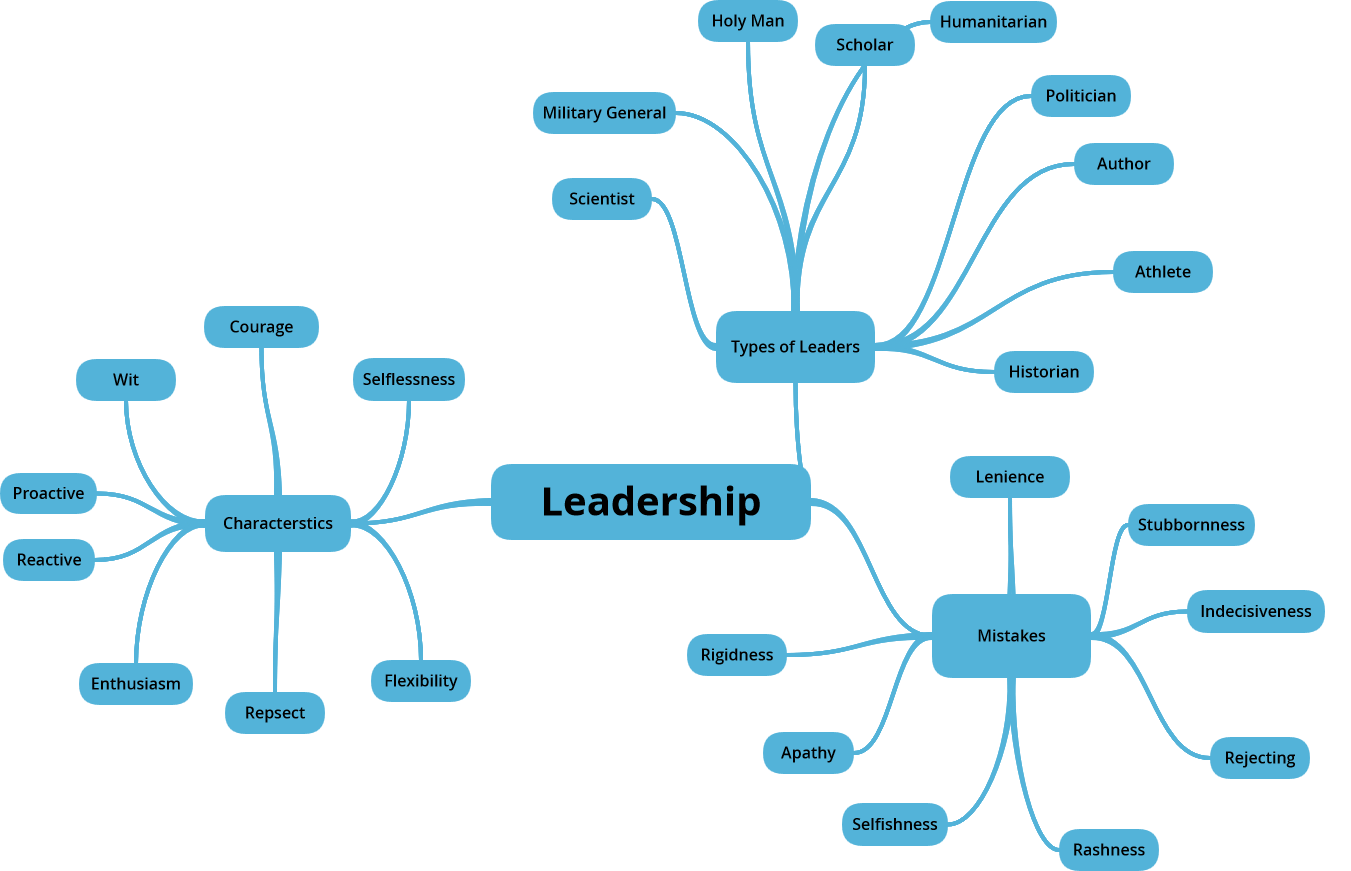
\includegraphics[scale=0.07]{images/mindmap.png}\\
 \vspace{0.5cm}

\includegraphics[scale=0.1]{images/black.png}

\includegraphics[scale=0.04]{images/list.png}

\includegraphics[scale=0.1]{images/black.png}

\includegraphics[scale=0.09]{images/srd.png}
 
\includegraphics[scale=0.1]{images/black.png}

\includegraphics[scale=0.07]{images/logo.png}


}


\frame{\frametitle{Done}
 \begin{multicols}{2}
    \begin{itemize}
      \item Brainstorming
      \item Learn Bitbucket, Trello and LaTeX
      \item Topic research
      \item Description of the project
      \item Functional requirements
      \item Non-Functional requirements
      \item Review and discussion of functional requirements
      \item Review and discussion of NFR
      \item Presentation
    \end{itemize}
  \end{multicols}

}

\section{Bitbucket}
\frame{\frametitle{Bitbucket}
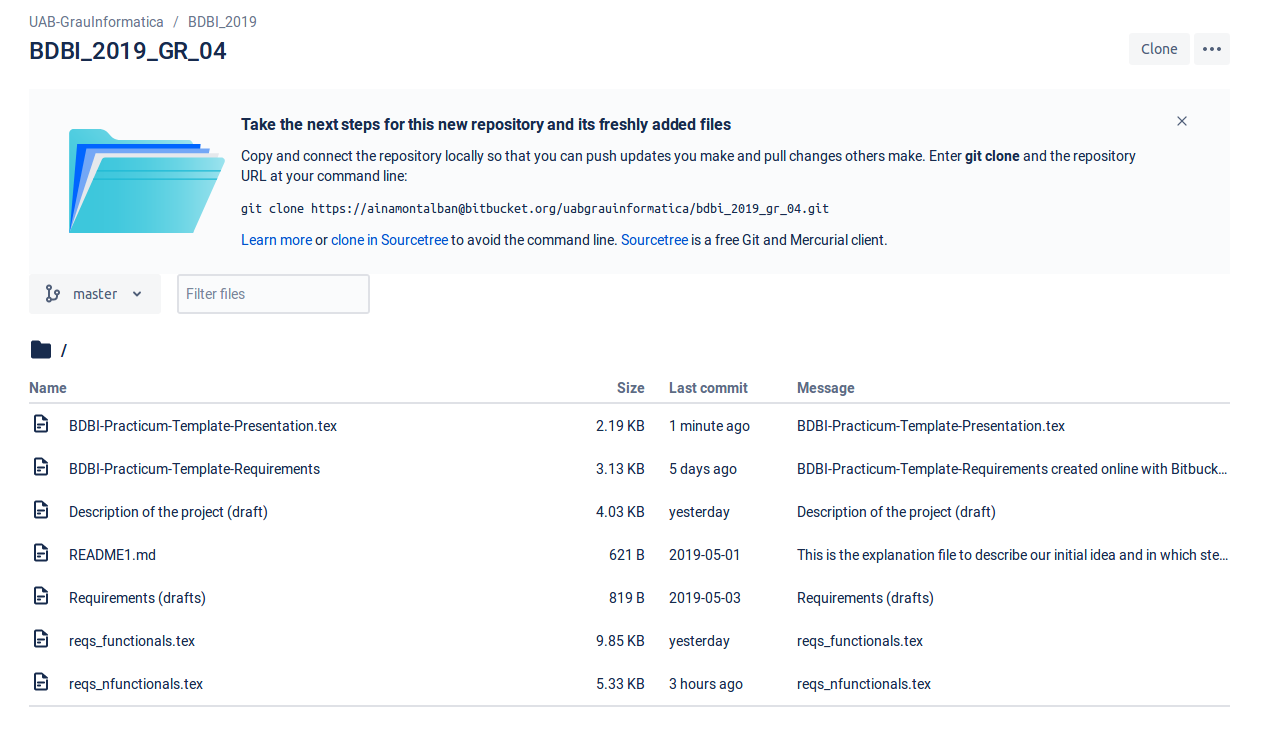
\includegraphics[scale=0.255]{images/bitbuck.png}
}

\section{Requeriments}
\subsection{Functional}
\frame{\frametitle{Requeriments}

\begin{itemize}
  \item The system shall manage a user login and register.\\
   \item The system will send an email if the user has forgotten the password with a new password. The user will need to introduce the email.\\
   \hspace{4cm}
  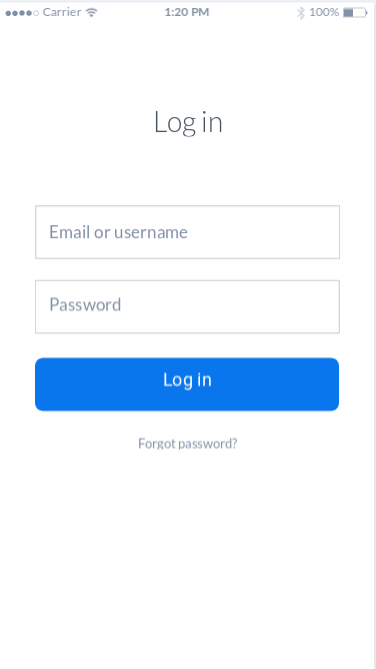
\includegraphics[scale=0.18]{images/login.png}

\end{itemize}
}

\frame{\frametitle{Requeriments}

\begin{itemize}
  \item A user shall be able to enter to a NA with a password.
  \item The user shall have a list of its NA and be able to select one of the NA.\\
  \vspace{0.5cm}
     \hspace{3cm}
   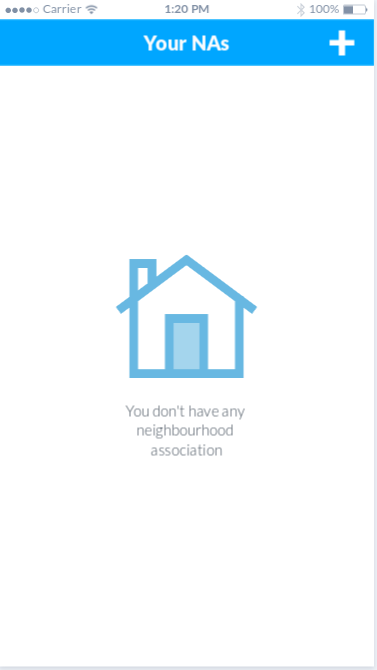
\includegraphics[scale=0.11]{images/NAs.png}
   \hspace{1cm}
  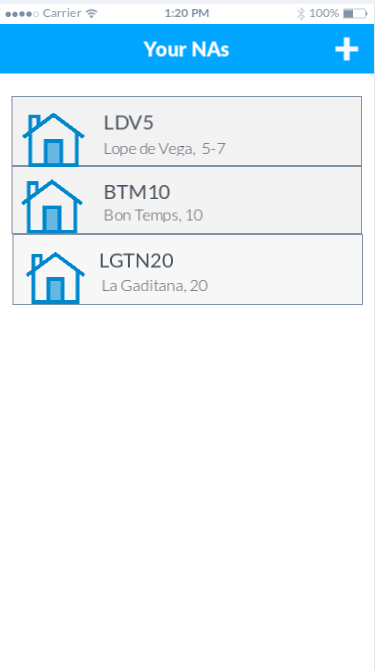
\includegraphics[scale=0.11]{images/na_list.png}

\end{itemize}
}

\frame{\frametitle{Requeriments}

\begin{itemize}
  \item The system shall use a instant messaging system to send messages to all the neighbours.
  \item The user shall be able to add warnings.
  %\item The user shall be able to introduce meetings or activities in the calendar.
  \item The system shall have free-text search, a text box where the user can introduce an string.\\
    \hspace{5cm}
   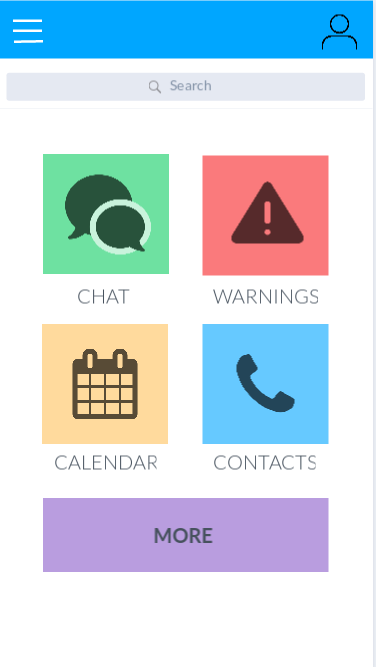
\includegraphics[scale=0.15]{images/user.png}

\end{itemize}
}

\frame{\frametitle{Requeriments}
\begin{itemize}
  \item The system shall allow the PA to summon a meeting in the calendar.
  \item The PA shall be able to finance the payments of the community.\\
  \hspace{4cm}
     
\includegraphics[scale=0.18]{images/admin.png}
\end{itemize}}




\subsection{Non Functional}
\frame{\frametitle{Diagrama}

  \begin{figure}[ht]
  \centering
  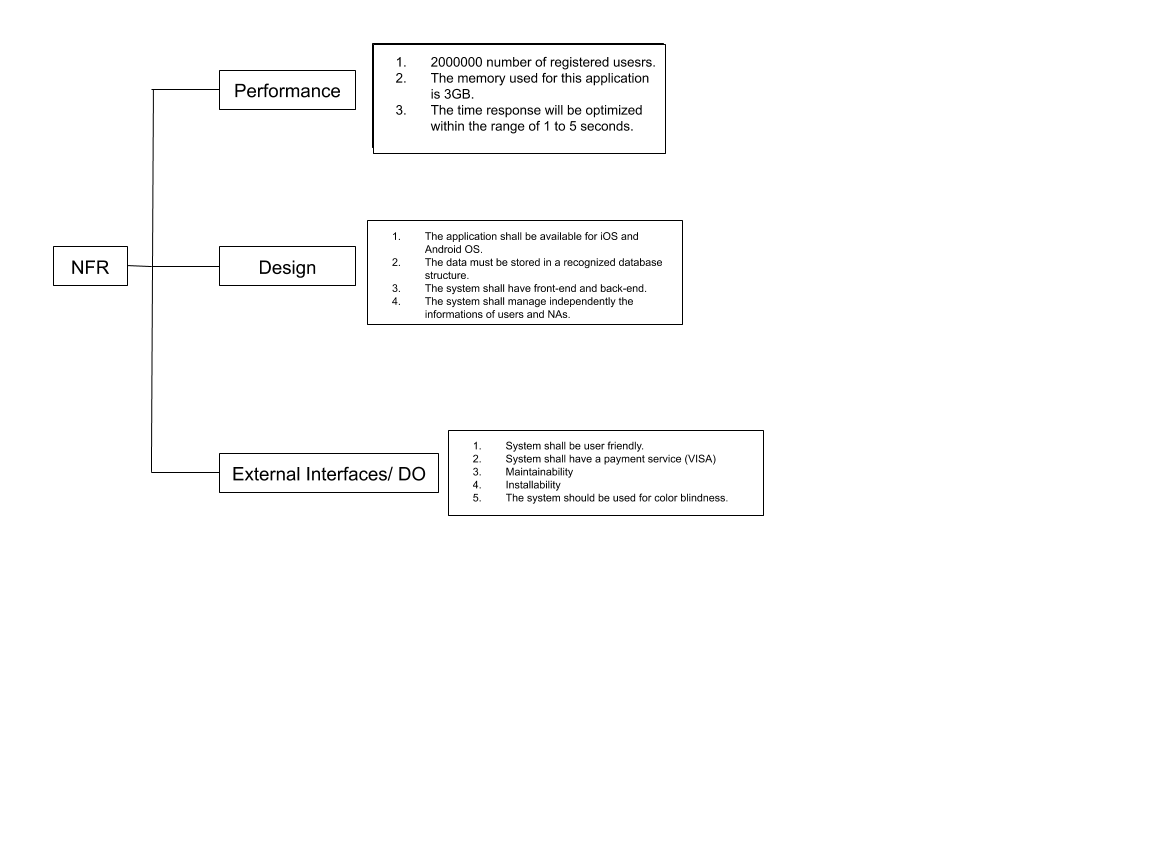
\includegraphics[width=1.1\textwidth]{images/rnf2.png}
  \label{fig:req}
   \end{figure}
}

\section{Conclusions}
\frame{\frametitle{Conclusions}
\begin{itemize}
    \item Usage of tools: trello and bitbucket (we'll keep trying...)
    \item A lot of requirements ---
         %
\includegraphics[scale=0.18]{admin.png}
\end{itemize}
}


\end{document}
